\subsection{latex}

\paragraph{TeXとは}
\begin{description}
\item 「テック」または「テフ」と読む,組版ソフト.
スタンフォード大学のDonald E.Knuth教授によって作られた.
他のソフトと組み合わせて,組版結果を画面や紙に出力したり,
PDF形式で出力したりする.参考文献5「LATEX2e 美文書作成入門」,奥村晴彦/黒木祐介著,技術評論社,2016,p.1-2
\end{description}

\paragraph{TeXの特徴}
\begin{itemize}
\item フリーソフトなので無料で入手でき,自由に中身を調べたり改良したりできる.
\item Windows,Mac,LinuxなどのOSに関わらず同じ動作をする.
\item TeXの文書はテキストファイルなので,普通のテキストエディタで読み書きでき,再利用やデータベース化が容易.
\item 数式をテキスト形式で表す標準となっている.
\end{itemize}

\paragraph{latexとは}
\begin{description}
\item 「ラテック」または「ラテフ」と読む.
DEC(現在のHP)のコンピュータ科学者Leslie Lamportによって機能強化されたTeX.
もとのTeXと同様にフリーソフトとして配布されている.
参考文献5「LATEX2e 美文書作成入門」,奥村晴彦/黒木祐介著,技術評論社,2016,p.3
\end{description}


「以下,元のintroduction」
また,デザインパターンも「プログラマが持っていた暗黙知に名前をつけることで形式知化した」と
ruby開発者のまつもとゆきひろも指摘している\verb|{{fn'デザインパターン,コード解説'}}|.
ある意味,暗黙知の形式知化をいかに効率よく行うかは知識共有の最大の目的とも言える.

このような暗黙知と形式知を提供するフォーマットはそれぞれの特徴を引き出すためにそれぞれ異なった
フォーマットで記述されている.

\begin{itemize}
\item 暗黙知は主にメモとして保存しやすいように単純なテキスト形式が取られる.
\item web発信においては,複雑な構文となるhyper textではなく,手軽にwebサイトを構築するwikiに対応したmark up言語が取られる.
\item 書籍としては,体裁,数式の綺麗さだけでなく,目次,索引,引用文献などの自動作成の観点からlatexで書かれることが多い.
\end{itemize}
しかし,それぞれを別々に書いていては,一箇所に修正があるとすべてのフォーマットに対して行う必要が出てくる.
これはプログラマの心得の核心をなす「DRY(Don't Repeat Yourself)」原則を
破ることとなる\verb|{{fn('pragmatic programmer')}}|.
プログラマはこれらの変換を自動化するコンバータを作成して,一箇所の修正によって
他のフォーマットでの修正に反映されるように,自動的に行うシステムを構築している.

本研究においては,図2に示した通り,西谷研で活用しているメモソフト
my\_help,wiki cloneのhiki, およびlatexの間を自動変換するシステムの開発を目的としている.

\begin{figure}[htbp]\begin{center}
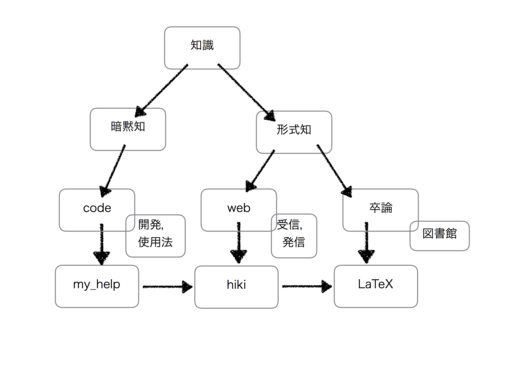
\includegraphics[width=6cm,bb=0 0 600  500]{knowledge_controll_cui.png}
\caption{知識の分類と,それぞれに適合したシステムおよびフォーマット.}
\label{default}\end{center}\end{figure}